\documentclass[a4paper,11pt]{article}
\usepackage[margin=1in]{geometry}
\usepackage{tikz,tkz-graph,graphicx}
\usepackage{xcolor}
\usetikzlibrary{arrows.meta,positioning,shapes}

% defining color is not necessary

\definecolor{lightOrange}{rgb}{0.9921875,0.890625,0.69921875}
\definecolor{darkOrange}{rgb}{0.96875,0.64453125,0.33203125}

\begin{document}

\section*{Picture}
\begin{figure}[h]
    \centering
    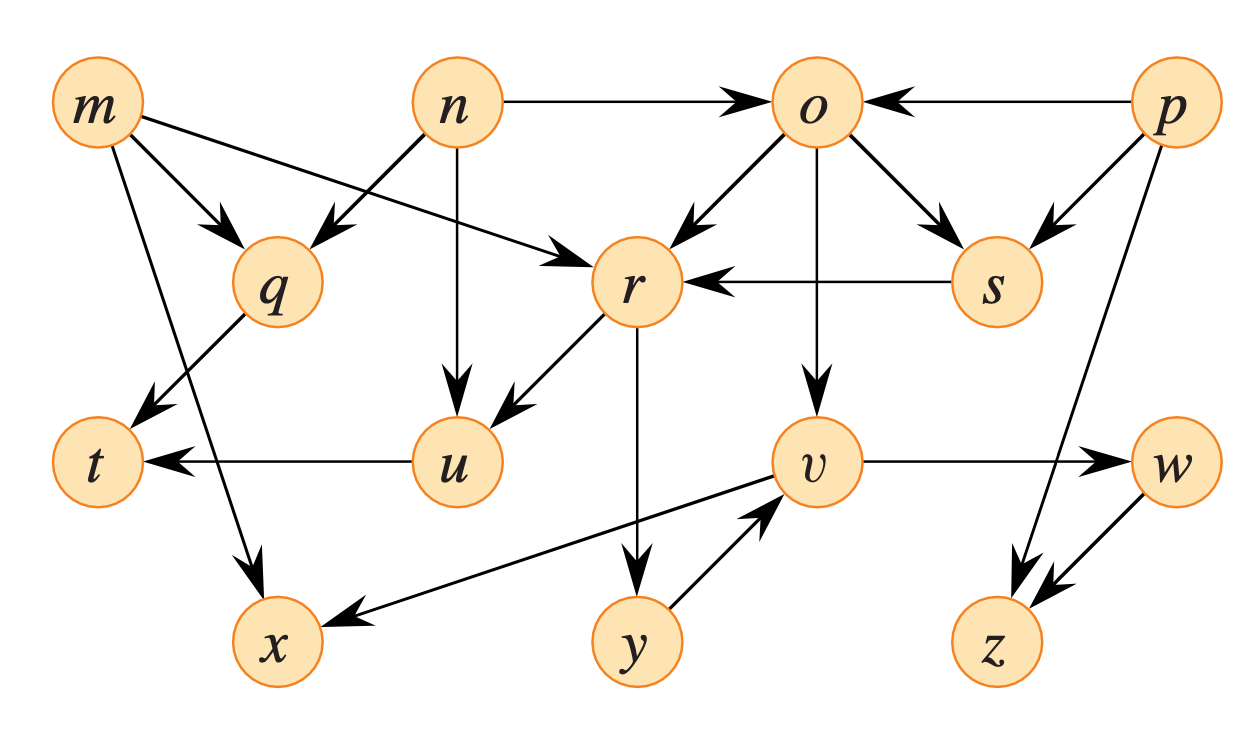
\includegraphics[width=0.7\textwidth]{./2.png}
\end{figure}

\section*{PDF}
\begin{figure}[th]
\centering
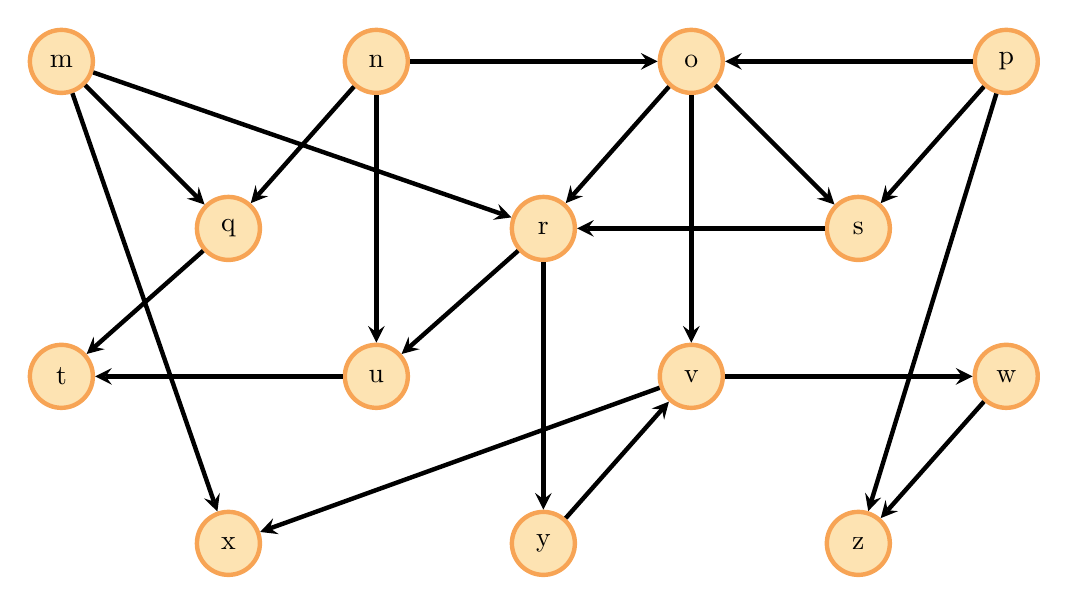
\begin{tikzpicture}[auto,main node/.style={circle,minimum size=8mm, draw=darkOrange,fill=lightOrange},scale=2,>=stealth,node distance=4cm,ultra thick]
    \node[main node] (m) [] {m};
    \node[main node] (n) [right of=m] {n};
    \node[main node] (o) [right of=n] {o};
    \node[main node] (p) [right of=o] {p};
    \node[main node] (t) [below of=m,node distance=4cm] {t};
    \node[main node] (u) [right of=t] {u};
    \node[main node] (v) [right of=u] {v};
    \node[main node] (w) [right of=v] {w};
    \node[main node] (q) [below right of=m,node distance=3cm] {q};
    \node[main node] (r) [right of=q] {r};
    \node[main node] (s) [right of=r] {s};
    \node[main node] (x) [below right of=t,node distance=3cm] {x};
    \node[main node] (y) [right of=x] {y};
    \node[main node] (z) [right of=y] {z};
    
    \path [->] (m) edge (q);
    \path [->] (m) edge (r);
    \path [->] (m) edge (x);
    \path [->] (n) edge (q);
    \path [->] (n) edge (u);
    \path [->] (n) edge (o);
    \path [->] (o) edge (r);
    \path [->] (o) edge (s);
    \path [->] (o) edge (v);
    \path [->] (p) edge (o);
    \path [->] (p) edge (s);
    \path [->] (p) edge (z);
    \path [->] (q) edge (t);
    \path [->] (r) edge (u);
    \path [->] (r) edge (y);
    \path [->] (s) edge (r);
    \path [->] (u) edge (t);
    \path [->] (v) edge (x);
    \path [->] (v) edge (w);
    \path [->] (w) edge (z);
    \path [->] (y) edge (v);  
\end{tikzpicture}
\end{figure}

\end{document}
